\documentclass{beamer}
\usetheme{Frankfurt}
\addtobeamertemplate{navigation symbols}{}{%
    \usebeamerfont{footline}%
    \usebeamercolor[fg]{footline}%
    \hspace{1em}%
    \insertframenumber/\inserttotalframenumber
}

\usepackage{mathtools}
\usepackage{graphicx}
\usepackage{braket}
\usepackage{amsthm}
\usepackage{lmodern}
\usepackage[utf8]{inputenc}
\usepackage[frenchb]{babel}
\usepackage[T1]{fontenc}
\usepackage{subcaption}
\usepackage{caption}
\usepackage{gensymb}
\usepackage{tikz}
\usepackage[qm]{qcircuit}
\usepackage{listings}
\usepackage{pgfplots}
\usepackage{xcolor}
\usepackage{amsmath}
\usepackage[ruled,vlined]{algorithm2e}
\captionsetup[figure]{labelformat=empty}

\definecolor{mGreen}{rgb}{0,0.6,0}
\definecolor{mGray}{rgb}{0.5,0.5,0.5}
\definecolor{mPurple}{rgb}{0.58,0,0.82}
\definecolor{backgroundColour}{rgb}{0.95,0.95,0.92}

\lstdefinestyle{CStyle}{
    backgroundcolor=\color{backgroundColour},   
    commentstyle=\color{mGreen},
    keywordstyle=\color{magenta},
    numberstyle=\tiny\color{mGray},
    stringstyle=\color{mPurple},
    basicstyle=\footnotesize,
    breakatwhitespace=false,         
    breaklines=true,                 
    captionpos=b,                    
    keepspaces=true,                 
    numbers=left,                    
    numbersep=5pt,                  
    showspaces=false,                
    showstringspaces=false,
    showtabs=false,                  
    tabsize=2,
    language=Python
}


\newtheorem{pb}{Problème}
\newtheorem{rem}{Remarque}
\newtheorem{ex}{Exemple}
%\newtheorem{definition}{Définition}

\titlegraphic{}

\title{Soutenance de rapport bibliographique - Informatique quantique}
\author{Pierre Engelstein}
\institute{Polytech Angers}

\begin{document}

%====================================
%================1===================

% \frame{\titlepage}

\makeatletter
\newcommand\titlegraphicii[1]{\def\inserttitlegraphicii{#1}}
\titlegraphicii{}
\setbeamertemplate{title page}
{
  \vbox{}
   {\usebeamercolor[fg]{titlegraphic}\inserttitlegraphic\hfill\inserttitlegraphicii\par}
  \begin{centering}
    \begin{beamercolorbox}[sep=8pt,center]{institute}
      \usebeamerfont{institute}\insertinstitute
    \end{beamercolorbox}
    \begin{beamercolorbox}[sep=8pt,center]{title}
      \usebeamerfont{title}\inserttitle\par%
      \ifx\insertsubtitle\@empty%
      \else%
        \vskip0.25em%
        {\usebeamerfont{subtitle}\usebeamercolor[fg]{subtitle}\insertsubtitle\par}%
      \fi%     
    \end{beamercolorbox}%
    \vskip1em\par
    \begin{beamercolorbox}[sep=8pt,center]{date}
      \usebeamerfont{date}\insertdate
    \end{beamercolorbox}%\vskip0.5em
    \begin{beamercolorbox}[sep=8pt,center]{author}
      \usebeamerfont{author}\insertauthor
    \end{beamercolorbox}
  \end{centering}
  %\vfill
}
\makeatother
\author{Pierre Engelstein}
\subtitle{\small Informatique quantique}
\title{\tiny Soutenance de rapport bibliographique}
\institute{Masters 2 Systèmes Dynamiques et Signaux}
\date{\today}
\titlegraphic{
\includegraphics[width=2cm]{../Rapport/images/LogoUnivAngers.png}}
\titlegraphicii{
\includegraphics[width=2cm]{../Rapport/images/Polytech_Angers.png}}

\begin{frame}[plain]
  \maketitle
  \tiny
  {\centering\itshape Membres du jury\par}
  Président: Pr. Laurent Hardouin\par\medskip
  \begin{tabular}[t]{@{}l@{\hspace{3pt}}p{.32\textwidth}@{}}
  Examinateurs: & Dr. Nicolas Delanoue \\
  & Pr. François Chapeau-Blondeau \\
  & Pr. Sébastien Lahaye \\
  & Dr. Mehdi Lhommeau \\
  & Pr. David Rousseau
  \end{tabular}%
  \footnotesize
  \tiny
  \begin{tabular}[t]{@{}l@{\hspace{3pt}}p{.3\textwidth}@{}}
  Encadrants : & Dr. Nicolas Delanoue \\
   & Pr. François Chapeau-Blondeau
  \end{tabular}%
\end{frame}


% Phrases bien cadrées sur l'introduction
% -> Performances de traitement de l'information inaccessibles en classique
% -> Trois algorithme quantiques qui illustrent cette performance
% -> 


\begin{frame}
  \tableofcontents
\end{frame}


%====================================
%====================================

% 4 minutes
\section[3 principes]{Les 3 principes de base pour l'informatique quantique}

% Dire que 3 principes de base: qubit, mesure, dynamique

\begin{frame}
\frametitle{3 Postulats}

\begin{enumerate}
  \item L'état d'un système quantique
  \item La dynamique d'un système quantique
  \item La mesure d'un système quantique
\end{enumerate}

\medbreak
Références bibliographiques: \cite{Nielsen00, Mermin07, Bennett98}
\end{frame}

% 2 minutes
\begin{frame}
\frametitle{ Postulat 1 : \'Etat d'un système quantique}
\only<1>{
\begin{block}{Définition} % Changer de "definition" à "définition"
  Système quantique: vecteur d'état $\ket{\psi}$ 
  
  \begin{itemize}
    \item dans un espace de Hilbert complexe $\mathcal{H}$,
    \item de norme unité: $||\psi||^2 = 1$,
    \item avec des coordonnées: \begin{equation} \ket{\psi} = \displaystyle\sum_{i} c_i \ket{k_i}, \end{equation}
    \item où $\{\ket{k_i}\}_i$ une base orthonormée de $\mathcal{H}$,
    \item et les coefficients $c_i \in \mathbb{C}$.
  \end{itemize}

\end{block}
}
% On représente l'état d'un système quantique au moyen d'un vecteur d'état psi appartenant à un espace de Hilbert complexe. Vecteur d'état étant de norme unité.

% Rajouter un exemple

\only<2>{
  Système quantique élémentaire: le qubit : $\ket{\psi} = \alpha \ket{0} + \beta \ket{1}$, dans un espace de Hilbert de dimension $2$. 

  %Element fondamental de l'informatique quantique.
\medbreak
% Définir bien le qubit comme étant l'élément fondamental de l'informatique quantique

\begin{example}
  \begin{equation}
    \ket{\psi_1} = \frac{1}{\sqrt{2}} \ket{0} + \frac{1}{\sqrt{2}} \ket{1},
  \end{equation}
  avec
  \begin{equation}
    \begin{bmatrix}
      1 \\ 0
    \end{bmatrix} \text{coordonnées de} \ket{0} 
     \text{et}
    \begin{bmatrix}
      0 \\ 1
    \end{bmatrix} \text{coordonnées de} \ket{1}.
  \end{equation}
\end{example}
}
\end{frame}

% 1 minute
\begin{frame}
  \frametitle{Postulat 2: Dynamique des systèmes quantiques}

  \begin{block}{Définition}
    La dynamique des systèmes quantiques respecte deux principes:
    \begin{list}{}
      \item - Conservation de la norme unité
      \item - Linéarité de l'évolution
    \end{list}
  \end{block}

  \begin{block}{Avec un système de coordonnées}
    Une évolution du système est donnée par une matrice $U$, telle que: $U^{\dagger}U = UU^{\dagger} = I$
  \end{block}

  %Opérateur unitaire (définition comme dans le rapport), => rédiger ici!!! TODO
  % Vision: état quantique en entrée, opérateur unitaire "boite noire" qui sort un état quantique de sortie. Vision fonction de transfert
\end{frame}


\begin{frame}
  \frametitle{Portes quantiques}

  \only<2>{

    \begin{block}{Exemple}
  Porte de Hadamard:
  \[
    H = \frac{1}{\sqrt{2}} \begin{bmatrix}
      1 & 1 \\
      1 & -1 \\
    \end{bmatrix}
  \]
  \end{block}

  \begin{block}{}
    Soit $\ket{\psi} = \ket{0} = \begin{bmatrix} 1 \\ 0 \\\end{bmatrix}$, alors $H\ket{\psi} = \begin{bmatrix}
      \frac{1}{\sqrt{2}} \\
      \frac{1}{\sqrt{2}} \\
    \end{bmatrix}$
  \end{block}
  }
  \only<1>{
    \begin{block}{Exemple}
    Porte de Pauli X :
    \[
      X = \begin{bmatrix}
        0 & 1 \\
        1 & 0 \\
      \end{bmatrix}
    \]
  \end{block}
    \begin{block}{}
      Soit $\ket{\psi} = \ket{0} = \begin{bmatrix} 1 \\ 0 \\\end{bmatrix}$, alors $X\ket{\psi} = \begin{bmatrix}
        0 \\
        1 \\
      \end{bmatrix} = \ket{1}$
    \end{block}
    \begin{block}{Remarque}
      La porte de Pauli X est l'équivalent de la porte \texttt{NON}
    \end{block}
    }



\end{frame}


% 1 minute
\begin{frame}
\frametitle{Postulat 3: La mesure projective}
\begin{definition}
  Quand un système quantique est dans un état $\ket{\psi} = \displaystyle\sum_{i} c_i \ket{k_i}$, on va avoir comme probabilité $|c_i|^2$ de mesurer l'état $\ket{k_i}$.
\end{definition}

\begin{rem}
  La mesure est \textbf{projective}: on pert l'état probabiliste.
\end{rem}

% Choix de la base projective (à noter ?)

\end{frame}

%====================================
%====================================
\section{3 algorithmes quantiques}

% Propriétés spécifiquement quantiques, montrent les apports spécifiques du quantique pour le traitement de l'information, permettent d'obtenir des performances inatteignables en classiques.

% 4 minutes
\subsection{Algorithme de Deutsch-Jozsa}

% 2 minutes
\begin{frame}
\frametitle{Algorithme de Deutsch-Jozsa \cite{Deutsch92}}

\begin{pb}
  Déterminer en le moins d'itérations possibles si une fonction $f$ booléenne est constante ou équilibrée
\end{pb}

\medbreak
Dans le cas classique: $2^{n-1} + 1$ itérations

\medbreak
Dans le cas quantique: 1 seule itération

\end{frame}

% 2 minutes
\begin{frame}
\frametitle{Algorithme}

\begin{figure}[htbp]
  \centering
  \centerline{
      \Qcircuit @C=1em @R=.7em {
        & \lstick{\ket{0}^n} \barrier[-1.75em]{1} & \gate{H^{\otimes n}} \barrier[-1.5em]{1} & \multigate{1}{U_f} \barrier[-1.75em]{1} & \gate{H^{\otimes n}} \barrier[-1.5em]{1} & \meter \\
        & \lstick{\ket{1}} & \gate{H} & \ghost{U_f} & \qw & \\
        \hspace{3em} \ket{u_{0}} & \hspace{9em} \ket{u_{1}} &  \hspace{10em} \ket{u_{2}} & \hspace{10em} \ket{u_{3}}
      }
  }
  \label{fig:univerise}
\end{figure}

\begin{enumerate}
  \item Initialisation: $\ket{u_0}$
  \item $\ket{u_1}$: Mise à l'équilibre: porte de Hadamard
  \item $\ket{u_2}$: Application de la fonction $U_f$
  \item $\ket{u_3}$: Préparation pour la mesure
\end{enumerate}

\end{frame}

%====================================
%====================================

% 4 minutes

\subsection{Algorithme de Grover}
% 1 minutes
\begin{frame}
\frametitle{Algorithme de Grover \cite{Grover96}}

\begin{pb}
  On souhaite chercher une entrée spécifique dans une liste non triée à N éléments de façon efficace.
\end{pb}

\medbreak
Dans le cas classique: $N$ itération successives.
\medbreak
Dans le cas quantique: $\mathcal{O}(\sqrt{N})$

\end{frame}

% 2 minutes
\begin{frame}
\frametitle{Opérateur de grover}
\begin{columns}
\begin{column}{0.5\textwidth}
  \only<1,2,3>{
\begin{figure}[htbp]
  \centering
  \centerline{
      \Qcircuit @C=1em @R=.7em {
        & \lstick{\ket{0}^n} \barrier[-1.75em]{1}  & \gate{H^{\otimes n}} \barrier[-1.75em]{1} & \multigate{1}{U_w} \barrier[-1.5em]{1} & \multigate{1}{U_s} \barrier[-1.25em]{1} & \meter \\
        & \lstick{\ket{1}} & \gate{H} & \ghost{U_w} &  \ghost{U_s} & \qw & \\
        \hspace{3em} \ket{u_{0}} & \hspace{8em} \ket{u_{1}} &  \hspace{10em} \ket{u_{2}} & \hspace{10em} \ket{u_{3}}
      }
    }
  \caption{Schéma du circuit de l'algorithme de Grover}
  \label{fig:grover}
\end{figure}
  }

\end{column}


\pgfplotstableread[row sep=\\,col sep=&]{
    state & amplitude \\
    $\ket{000}$ & 0.35355  \\
    $\ket{001}$ & 0.35355  \\
    $\ket{010}$ & 0.35355  \\
    $\ket{011}$ & 0.35355  \\
    $\ket{100}$ & 0.35355  \\
    $\ket{101}$ & 0.35355  \\
    $\ket{110}$ & 0.35355  \\
    $\ket{111}$ & 0.35355  \\
}\afterHadamard
\pgfplotstableread[row sep=\\,col sep=&]{
    state & amplitude \\
    $\ket{000}$ & 0.35355  \\
    $\ket{001}$ & 0.35355  \\
    $\ket{010}$ & -0.35355  \\
    $\ket{011}$ & 0.35355  \\
    $\ket{100}$ & 0.35355  \\
    $\ket{101}$ & 0.35355  \\
    $\ket{110}$ & 0.35355  \\
    $\ket{111}$ & 0.35355  \\
}\afterUw
\pgfplotstableread[row sep=\\,col sep=&]{
    state & amplitude \\
    $\ket{000}$ & 0.176  \\
    $\ket{001}$ & 0.176  \\
    $\ket{010}$ & 0.884  \\
    $\ket{011}$ & 0.176  \\
    $\ket{100}$ & 0.176  \\
    $\ket{101}$ & 0.176  \\
    $\ket{110}$ & 0.176  \\
    $\ket{111}$ & 0.176  \\
}\afterUs


\begin{column}{0.5\textwidth}
\only<1>{
\begin{figure}[t]{}
  \centering
  \begin{tikzpicture}[scale=0.55]
    \begin{axis}[
            ybar,
            symbolic x coords={$\ket{000}$, $\ket{001}$, $\ket{010}$, $\ket{011}$, $\ket{100}$, $\ket{101}$, $\ket{110}$, $\ket{111}$},
            xtick=data,
        ]
        \addplot table[x=state,y=amplitude]{\afterHadamard};
    \end{axis}
  \end{tikzpicture}
%     \label{fig:groverAmp}
    \caption{$\ket{u_1}$}
\end{figure}
}
\only<2>{
\begin{figure}[b]{}
    \centering
    \begin{tikzpicture}[scale=0.55]
      \begin{axis}[
              ybar,
              symbolic x coords={$\ket{000}$, $\ket{001}$, $\ket{010}$, $\ket{011}$, $\ket{100}$, $\ket{101}$, $\ket{110}$, $\ket{111}$},
              xtick=data,
          ]
          \addplot table[x=state,y=amplitude]{\afterUw};
      \end{axis}
      \draw[line width=0.1 mm] (0,4.6) -- (6.85,4.6);
    \end{tikzpicture}
    \caption{$\ket{u_2}$}
\end{figure}
}
\only<3>{
\begin{figure}[b]
  \centering
  \begin{tikzpicture}[scale=0.55]
    \begin{axis}[
            ybar,
            symbolic x coords={$\ket{000}$, $\ket{001}$, $\ket{010}$, $\ket{011}$, $\ket{100}$, $\ket{101}$, $\ket{110}$, $\ket{111}$},
            xtick=data,
        ]
        \addplot table[x=state,y=amplitude]{\afterUs};
    \end{axis}
  \end{tikzpicture}
  \caption{$\ket{u_3}$}
\end{figure}
}


% \only<4>{
%   \begin{figure}[h]
%     \centering
%     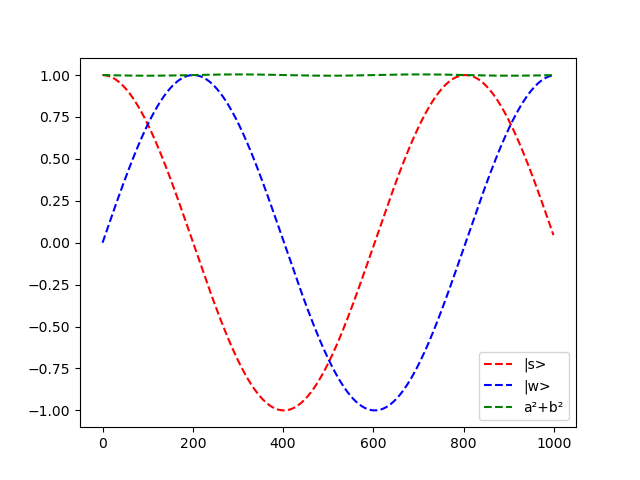
\includegraphics[scale=0.3]{../Rapport/images/Grover/grover_n16_1000.png}
%     \caption{Evolution des modules pour n=16, sur 1000 itérations}
%     \label{fig:groverGraph}
%   \end{figure}
% }

\end{column}

\end{columns}

\only<4>{
  \begin{figure}[htbp]
    \centering
    \centerline{
        \Qcircuit @C=1em @R=.7em {
          & & & & \mbox{$\mathcal{O}(\sqrt N)$ itérations} \\
          & \lstick{\ket{0}^n} \barrier[-1.75em]{1}  & \gate{H^{\otimes n}} \barrier[-1.75em]{1} & \multigate{1}{U_w} \barrier[-1.5em]{1} & \multigate{1}{U_s} \barrier[-1.25em]{1} & \meter \\
          & \lstick{\ket{1}} & \gate{H} & \ghost{U_w} &  \ghost{U_s} & \qw & \\
          \hspace{3em} \ket{u_{0}} & \hspace{8em} \ket{u_{1}} &  \hspace{10em} \ket{u_{2}} & \hspace{10em} \ket{u_{3}} \gategroup{2}{4}{3}{5}{.7em}{^\}}
        }
      }
    \caption{Schéma du circuit de l'algorithme de Grover}
    \label{fig:grover}
  \end{figure}
}
\end{frame}

%====================================
%====================================
\subsection{Algorithme de Shor}

\begin{frame}
\frametitle{Algorithme de Shor \cite{Shor97}}

Problème de factorisation de grands entiers en nombres premiers: résoudre $N = p \times q$ avec $p$ et $q$ entiers très grands inconnus. 

\medbreak

- Algorithmes classiques: complexité exponentielle
\medbreak
- Algorithmes quantiques: complexité polynomiale

% Dans les grandes lignes

% Algorithmes classiques: complexité exponentielle
% Algorithme quantique: complexité polynomiale

% On montre que le problème de factorisation se converti en recherche de période abordé par la tranformée de Fourier quantique.

\end{frame}

\section{Pistes de recherche (pour le stage)}
% Grandes pistes de recherche
% Pistes pour le stage
\begin{frame}
  \frametitle{Travail à venir}
  % -> Par ex DJ extension à autres catégories

  \begin{enumerate}
    \item \'Etendre Deutsch-Jozsa à d'autres problèmes (exemple de Bernstein-Vazirani)
    \item Optimalité de la décomposition en portes élémentaires \texttt{CNOT}
  \end{enumerate}

\end{frame}

% 2 minutes
\section{Conclusion}
\begin{frame}
\frametitle{Conclusion}

Domaine de recherche actif, en plein essort.

\medbreak

De nombreuses entreprises se positionnent dessus: IBM, Microsoft, Google, Intel, Atos.

% -> Domaine très riche en plein essort, plein de boites se positionnent dessus, plein de labos
\end{frame}

\begin{frame}
\frametitle{Bibliographie}

\tiny
\bibliographystyle{ieeetr}
\bibliography{biblio}

% -> Refs sur la base (1-2 refs), par exemple IEEE et livres de cours
% -> Ref pour DJ, Grover et Shor
% -> Refs sur les signaux IEEE ?
% Referencer vers la biblio avec bibtex ou juste un enumerate

% \begin{itemize}
%     % \fontsize{6pt}{7.2}\selectfont
%     % \item R. Buyya, R. N. Calheiros, J. Son, A. V. Dastjerdi and Y. Yoon, "Software-Defined Cloud Computing: Architectural elements and open challenges," 2014 International Conference on Advances in Computing, Communications and Informatics (ICACCI), New Delhi, 2014, pp. 1-12
%     % \item Bhore, Pratik. (2016). A Survey on Storage Virtualization and its Levels along with the Benefits and Limitations. INTERNATIONAL JOURNAL OF COMPUTER SCIENCES AND ENGINEERING. 4. 115-121.
%     % \item M. F. Bari et al., "Data Center Network Virtualization: A Survey," in IEEE Communications Surveys \& Tutorials, vol. 15, no. 2, pp. 909-928
%     % \item M. Alouane and H. El Bakkali, "Virtualization in Cloud Computing: Existing solutions and new approach," 2016 2nd International Conference on Cloud Computing Technologies and Applications (CloudTech), Marrakech, 2016, pp. 116-123
%     % \item Chrobak, Pawel. (2014). Implementation of Virtual Desktop Infrastructure in academic laboratories. 1139-1146.
%     % \item Nagesh, O \& Kumar, Tapas \& Venkateswararao, V.. (2017). A Survey on Security Aspects of Server Virtualization in Cloud Computing. International Journal of Electrical and Computer Engineering. 7. 1326-1336.
% \end{itemize}
\end{frame}

\end{document}
